\section{Tendência do Mercado}

\begin{frame}[fragile]{Hype Curve Technology}
\begin{figure}[ht!]
  \centering
  \includesvg[inkscapelatex=false, scale=0.32]{images/hype.svg}
\end{figure}
\begin{center}
\small{Como discernir o que é \textbf{hype} do que é \textbf{viável?}}
\end{center}
\end{frame}

\begin{frame}[fragile]{GitHub Octoverse 2018}
\begin{figure}[ht!]
  \centering
  \includegraphics[scale=0.3]{images/octoverse.png}
\end{figure}
\begin{center}
\small{GitHub tendências e insights}
\small{https://octoverse.github.com/}
\end{center}
\end{frame}

\begin{frame}[fragile]{Linguagens de 2018}

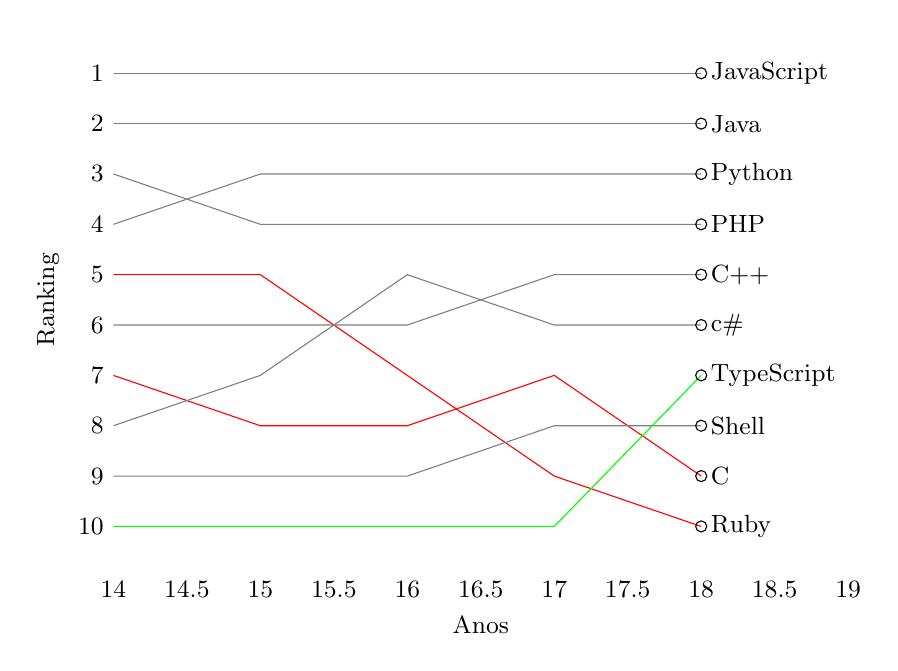
\begin{tikzpicture}[font=\small]
    \pgfplotsset{
        width=0.9\textwidth,
        height=0.7\textwidth
    }
	\begin{axis}[
	    y axis line style = { draw=none },
	    tickwidth = 0pt,
		xlabel=Anos,
		ylabel=Ranking,
		xmin=14,xmax=19,
		y dir=reverse,
        ytick distance=1
	]
	\addplot [mark=none, color=gray] coordinates {(14,1)(15,1)(16,1)(17,1)(18,1)};
	\addplot [mark=none, color=gray] coordinates {(14,2)(15,2)(16,2)(17,2)(18,2)};
	\addplot [mark=none, color=gray] coordinates {(14,4)(15,3)(16,3)(17,3)(18,3)};
	\addplot [mark=none, color=gray] coordinates {(14,3)(15,4)(16,4)(17,4)(18,4)};
	\addplot [mark=none, color=red] coordinates {(14,5)(15,5)(16,7)(17,9)(18,10)};
	\addplot [mark=none, color=gray] coordinates {(14,6)(15,6)(16,6)(17,5)(18,5)};
	\addplot [mark=none, color=red] coordinates {(14,7)(15,8)(16,8)(17,7)(18,9)};
	\addplot [mark=none, color=gray] coordinates {(14,8)(15,7)(16,5)(17,6)(18,6)};
	\addplot [mark=none, color=gray] coordinates {(14,9)(15,9)(16,9)(17,8)(18,8)};
	\addplot [mark=none, color=green] coordinates {(14,10)(15,10)(16,10)(17,10)(18,7)};
	
	\draw (axis cs:18,1) circle (2pt) node [right] {JavaScript};
	\draw (axis cs:18,2) circle (2pt) node [right] {Java};
	\draw (axis cs:18,3) circle (2pt) node [right] {Python};
	\draw (axis cs:18,4) circle (2pt) node [right] {PHP};
	\draw (axis cs:18,5) circle (2pt) node [right] {C++};
	\draw (axis cs:18,6) circle (2pt) node [right] {c\#};
	\draw (axis cs:18,7) circle (2pt) node [right] {TypeScript};
	\draw (axis cs:18,8) circle (2pt) node [right] {Shell};
	\draw (axis cs:18,9) circle (2pt) node [right] {C};
	\draw (axis cs:18,10) circle (2pt) node [right] {Ruby};
	
	\end{axis}
\end{tikzpicture}

\begin{center}
\small{Principais linguagens ao longo do tempo}
\end{center}
\end{frame}

\begin{frame}[fragile]{Linguagens com crescimento mais rápido}

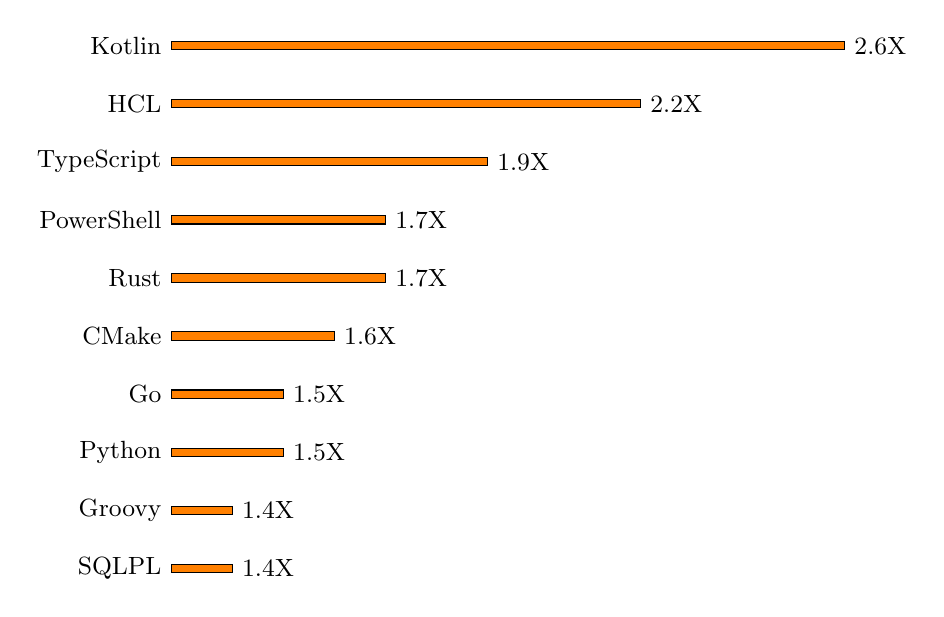
\begin{tikzpicture}[font=\small]
\pgfplotsset{
    width=0.9\textwidth,
    height=0.7\textwidth
}
\begin{axis}
[
    xbar,
    y axis line style = { draw=none },
    axis x line = none,
    tickwidth = 0pt,
    nodes near coords,
    nodes near coords={\pgfmathprintnumber\pgfplotspointmeta X},
    enlarge y limits=0.02,
    ytick distance=1,
    y dir=reverse,
    symbolic y coords = {
        Kotlin,
        HCL,
        TypeScript,
        PowerShell,
        Rust,
        CMake,
        Go,
        Python,
        Groovy,
        SQLPL
    },
]
    \addplot[
      fill=orange, 
      bar width=3pt, 
      label style={font=\small}, 
      tick label style={font=\small}
    ] coordinates { 
        (2.6,Kotlin)
        (2.2,HCL)
        (1.9,TypeScript)
        (1.7,PowerShell)
        (1.7,Rust)
        (1.6,CMake)
        (1.5,Go)
        (1.5,Python)
        (1.4,Groovy)
        (1.4,SQLPL) 
    };
  \end{axis}
\end{tikzpicture}

\begin{center}
\small{Tendências em direção a mais linguagens com tipos estáticos e interoperabilidade}
\end{center}
\end{frame}

\begin{frame}[fragile]{Stack Overflow}
\begin{figure}[ht!]
  \centering
  \includegraphics[scale=0.4]{images/stackoverflow.png}
\end{figure}
\begin{center}
\small{Quase 90.000 mil desenvolvedores profissionais participaram}
\small{https://insights.stackoverflow.com/survey/2019}
\end{center}

\end{frame}

\begin{frame}[fragile]{Linguagens mais populares}
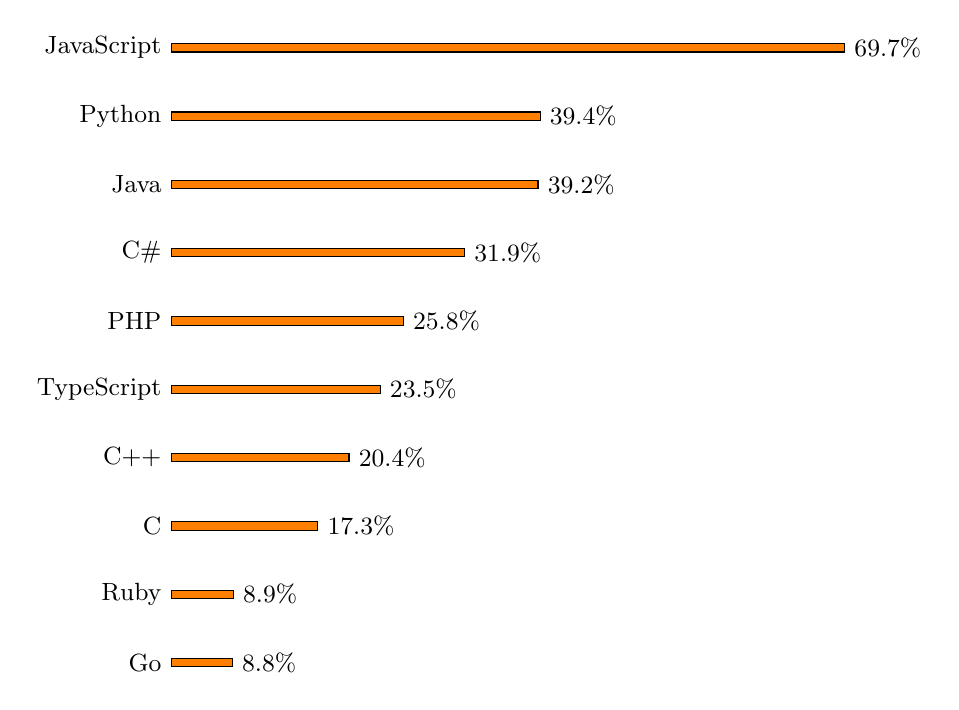
\begin{tikzpicture}[font=\small]
\pgfplotsset{
    width=0.9\textwidth,
    height=0.8\textwidth
}
\begin{axis}
[
    xbar,
    y axis line style = { draw=none },
    axis x line = none,
    tickwidth = 0pt,
    nodes near coords,
    nodes near coords={\pgfmathprintnumber\pgfplotspointmeta \%},
    enlarge y limits=0.02,
    ytick distance=1,
    y dir=reverse,
    symbolic y coords = {
        JavaScript,
        Python,
        Java,
        C\#,
        PHP,
        TypeScript,
        C++,
        C,
        Ruby,
        Go
    },
]
    \addplot[
      fill=orange, 
      bar width=3pt, 
      label style={font=\small}, 
      tick label style={font=\small}
    ] coordinates { 
        (69.7,JavaScript) 
        (39.4,Python) 
        (39.2,Java) 
        (31.9,C\#) 
        (25.8,PHP) 
        (23.5,TypeScript) 
        (20.4,C++) 
        (17.3,C) 
        (8.9,Ruby) 
        (8.8,Go)
    };
  \end{axis}
\end{tikzpicture}
\begin{center}
\small{Quais são as linguagens mais populares?}
\end{center}
\end{frame}

\begin{frame}[fragile]{Linguagens mais desejadas}
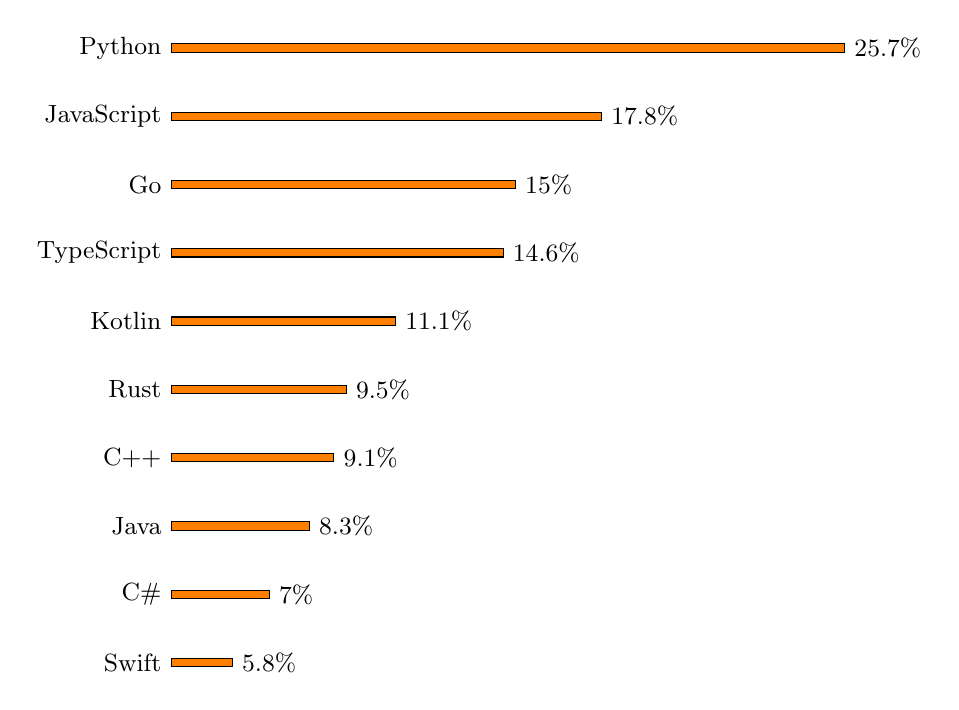
\begin{tikzpicture}[font=\small]
\pgfplotsset{
    width=0.9\textwidth,
    height=0.8\textwidth
}
\begin{axis}
[
    xbar,
    y axis line style = { draw=none },
    axis x line = none,
    tickwidth = 0pt,
    nodes near coords,
    nodes near coords={\pgfmathprintnumber\pgfplotspointmeta \%},
    enlarge y limits=0.02,
    ytick distance=1,
    y dir=reverse,
    symbolic y coords = {
        Python,
        JavaScript,
        Go,
        TypeScript,
        Kotlin,
        Rust,
        C++,
        Java,
        C\#,
        Swift
    },
]
    \addplot[
      fill=orange, 
      bar width=3pt, 
      label style={font=\small}, 
      tick label style={font=\small}
    ] coordinates { 
        (25.7,Python)
        (17.8,JavaScript)
        (15.0,Go)
        (14.6,TypeScript)
        (11.1,Kotlin)
        (9.5,Rust)
        (9.1,C++)
        (8.3,Java)
        (7.0,C\#)
        (5.8,Swift)
    };
  \end{axis}
\end{tikzpicture}
\begin{center}
\small{Qual linguagem você não usa e deseja aprender?}
\end{center}
\end{frame}

\begin{frame}[fragile]{Linguagens mais amadas}
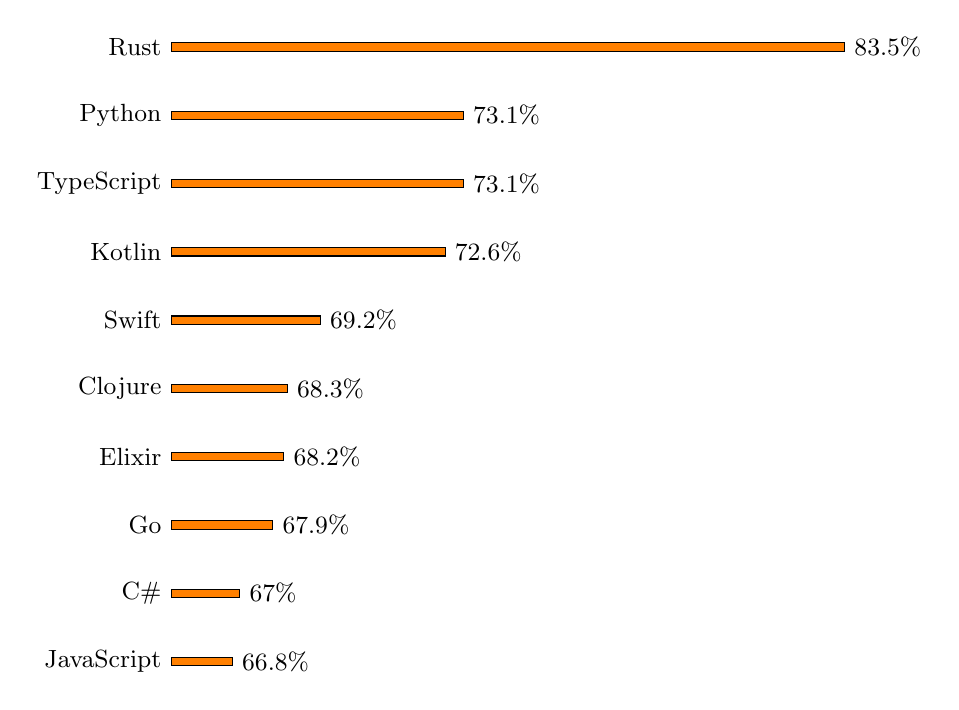
\begin{tikzpicture}[font=\small]
\pgfplotsset{
    width=0.9\textwidth,
    height=0.8\textwidth
}
\begin{axis}
[
    xbar,
    y axis line style = { draw=none },
    axis x line = none,
    tickwidth = 0pt,
    nodes near coords,
    nodes near coords={\pgfmathprintnumber\pgfplotspointmeta \%},
    enlarge y limits=0.02,
    ytick distance=1,
    y dir=reverse,
    symbolic y coords = {
        Rust,
        Python,
        TypeScript,
        Kotlin,
        Swift,
        Clojure,
        Elixir,
        Go,
        C\#,
        JavaScript
    },
]
    \addplot[
      fill=orange, 
      bar width=3pt, 
      label style={font=\small}, 
      tick label style={font=\small}
    ] coordinates { 
        (83.5,Rust)
        (73.1,Python)
        (73.1,TypeScript)
        (72.6,Kotlin)
        (69.2,Swift)
        (68.3,Clojure)
        (68.2,Elixir)
        (67.9,Go)
        (67.0,C\#)
        (66.8,JavaScript)
    };
  \end{axis}
\end{tikzpicture}

\begin{center}
\small{Qual linguagem você usa e deseja continuar?}
\end{center}
\end{frame}

\begin{frame}[fragile]{Linguagens mais temidas}
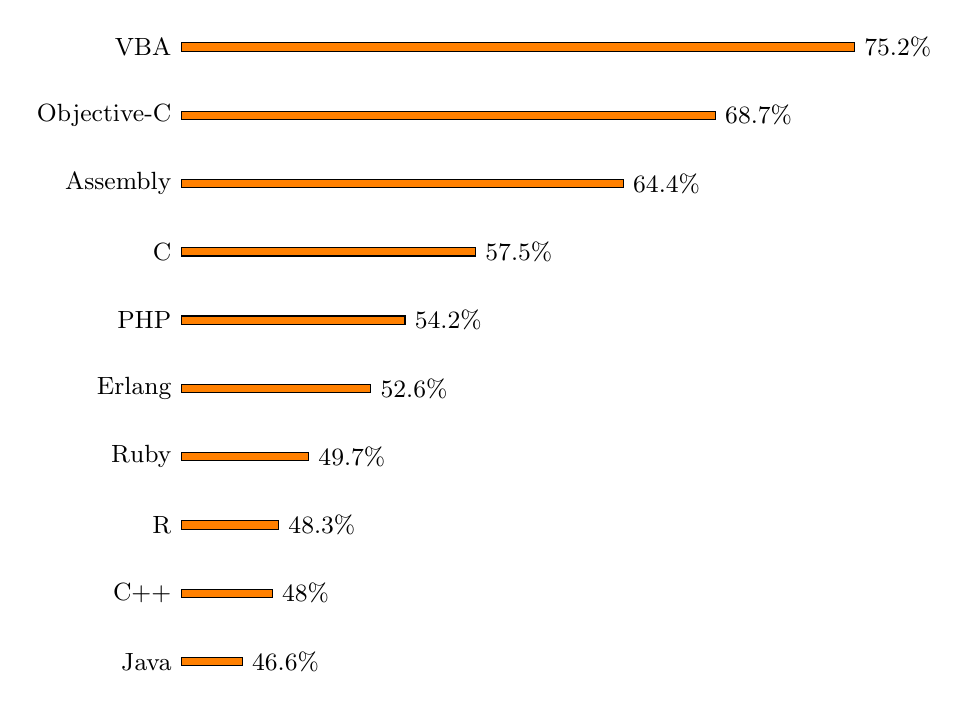
\begin{tikzpicture}[font=\small]
\pgfplotsset{
    width=0.9\textwidth,
    height=0.8\textwidth
}
\begin{axis}
[
    xbar,
    y axis line style = { draw=none },
    axis x line = none,
    tickwidth = 0pt,
    nodes near coords,
    nodes near coords={\pgfmathprintnumber\pgfplotspointmeta \%},
    enlarge y limits=0.02,
    ytick distance=1,
    y dir=reverse,
    symbolic y coords = {
        VBA,
        Objective-C,
        Assembly,
        C,
        PHP,
        Erlang,
        Ruby,
        R,
        C++,
        Java
    },
]
    \addplot[
      fill=orange, 
      bar width=3pt, 
      label style={font=\small}, 
      tick label style={font=\small}
    ] coordinates { 
        (75.2,VBA) 
        (68.7,Objective-C) 
        (64.4,Assembly) 
        (57.5,C) 
        (54.2,PHP) 
        (52.6,Erlang) 
        (49.7,Ruby) 
        (48.3,R) 
        (48.0,C++) 
        (46.6,Java)
    };
  \end{axis}
\end{tikzpicture}
\begin{center}
\small{Qual linguagem você usa e não quer continuar?}
\end{center}
\end{frame}

\begin{frame}[fragile]{Salário e experiência por linguagens}
\begin{figure}[ht!]
  \centering
  \includesvg[inkscapelatex=false, scale=0.55]{images/salary_language.svg}
\end{figure}
\begin{center}
\small{Salário | Experiência}
\end{center}
\end{frame}
